%\documentclass{beamer}
%\usetheme{Pittsburgh} 
\documentclass{scrartcl}

\usepackage[utf8]{inputenc}
\usepackage{default}
\usepackage[procnames]{listings}
\usepackage{graphicx}
%\usepackage[toc,page]{appendix}
\usepackage{caption}
\usepackage{hyperref}
\usepackage{color}
\usepackage{pdfpages}


%Bibliogrpahy?
\usepackage{bibentry}
%\nobibliography*
%\bibentry{ }


\begin{document}

\title{Assignment No. 3}
\subtitle{}
\author{
  Quignon, Christophe \\
  %Familyname, Name
} 
\date{\today}


\maketitle

\section{Read chapter 2 from Haykin’s book (2nd edition), starting from section 2.13 to end of
chapter, leaving out section 2.15 (PAC learning). Summarize or sketch your insights in
mind-map or an outline or a summary.
}
\begin{enumerate}
\setcounter{enumi}{12}
\item Statistical Nature of the Learning Process
	\begin{itemize}
	\item For every measurement there is an error $\epsilon$ which we assume to be zero mean and random occurrence.
	\item This error can be modelled with regression.
	\item We can not know the bias, only the variance of an error.
	\item the price for a small bias is a large variance.
	\item the bias can only be minimized by the design of the NN
	\end{itemize}
\item statistical learning theory
	\begin{itemize}
	\item A learning model has three components:
		\begin{itemize}
		\item The Environment (supplying input $x$)
		\item The teacher (supplying desired response $d$)
		\item The learning algorithm (Mapping $x$ to $d$)
		\end{itemize}
	\item There is a loss $L$ or discrepancy between the actual and the desired output
	\item The expected Loss is defined by the risk function $R(w)$
	\item With empirical risk minimization we can minimize the risk with respect to the weights $w$
	\item The VC dimension measures the capacity of the family of classification functions.
	\item the VC dim is a combinatorial concept that is unrelated to geometry
	\item The vc dim of a multilayered feedforward network with a sigmoid activation function is $O(W^{2})$, where $W$ is the number of free parameters.
	\item the training error is the frequency of errors during learning
	\item the generalization error is the frequency of error after training
	\item the generalization error is bound by the guaranteed risk
	\item the guaranteed risk depends on the confidence interval and the training error. 
	\item the guaranteed risk has minimum that can be found by structural risk minimization
	\end{itemize}
\item -

\item Summary and discussion
	\begin{itemize}
	\item The Darwinian selective learning model relies on principles of evolution
	\item The Darwinian selective learning model groups neurons in repertoires which compete
	\end{itemize}
\end{enumerate}

\section{Give the
VC dimension of the following hypothesis spaces in the x, y plane:
}

\subsection{$H_{r}$ = the set of all rectangles}
The VC dimension of all rectangles parallel to the axis is 4. There is a set of four points which we can shatter. Those are at (1, -1), (1, 1), (-1, 1), (-1, -1). However the set as before as one group with a point of the other group in the middle can not be shattered, because the outer four points build the bounding box. See Figure~\ref{fig:rectangle}

\begin{figure}
 \center
 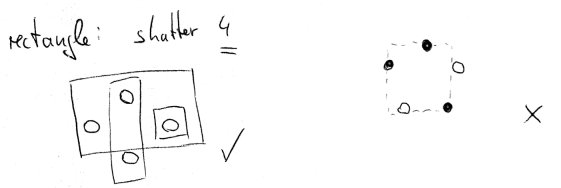
\includegraphics[width= 8cm]{vcdim_rectangle.jpg}
 \caption{Axis parallel rectangles have a VC dim of four.}
 \label{fig:rectangle}
\end{figure}

\subsection{$H_{c}$ = the set of all circles} 
The VC dimension of circles is three, because we can the set of (1, 2), (0, 2), (0, 0) can be shattered, while the set of {(0, 0), (0, 2)}, {(0, 1), 0, 3)} can not be shattered because the exclusion of the first and third point limit the size of the circle containing the second point. See Figure~\ref{fig:circle}.

\begin{figure}
 \center
 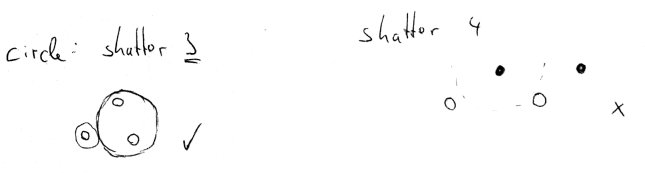
\includegraphics[width= 8cm]{vcdim_circle.jpg}
 \caption{Circles have a VC dim of three.}
 \label{fig:circle}
\end{figure}

\subsection{$H_{t}$ = the set of all triangles}
The VC dimension of triangles is 7. 7 Points on a circle can be shattered, because a set of four points can not limit a set of three points nor can a set of three points limit a set of four.\\
* alternating points on a circle however can not be shattered, because 4 rectangular points can not be enclosed by a triangle, if four alternated points enclose them. See Figure~\ref{fig:triangle}

\begin{figure}
 \center
 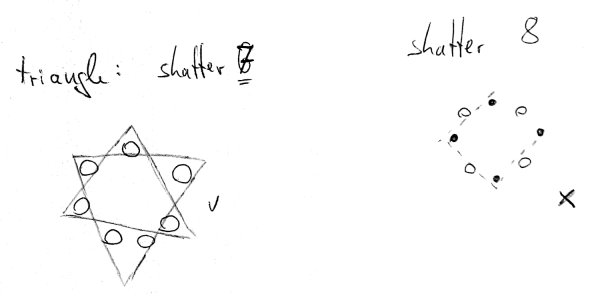
\includegraphics[width= 8cm]{vcdim_triangles.jpg}
 \caption{Triangles have a VC dim of 7}
 \label{fig:triangle}
\end{figure}

\section{Boltzmann learning}

$E = -\frac{1}{2}\Sigma_{j}\Sigma_{k}w_{k-j}x_{k}x_{j}$\\
$P(X_{k} \to -x_{k}) = \frac{1}{1+exp(-\Delta E_{k}/T)}$\\

Training = [(0, 1), (1, 0)]

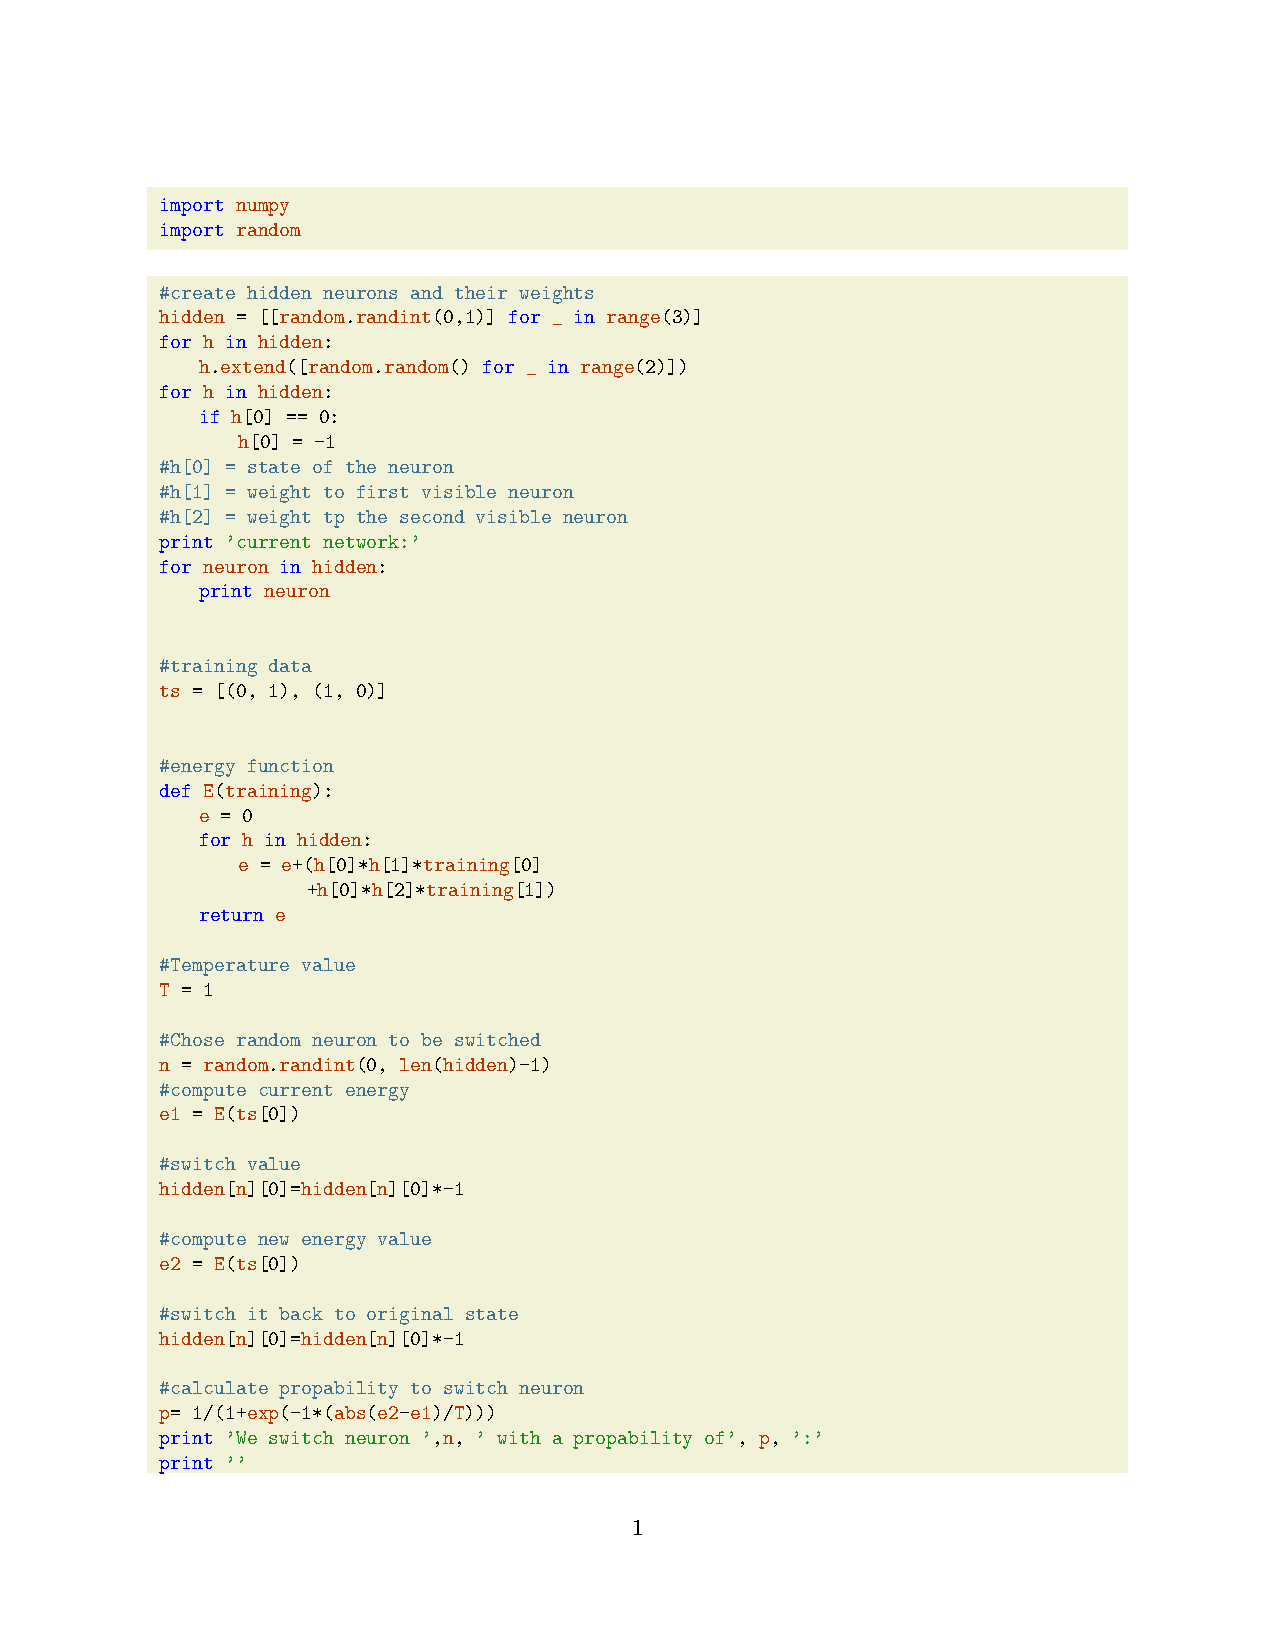
\includepdf[pages={1-},scale=1]{boltzmannweights.pdf}


\section{Please upload 3 questions and their brief answers on the reading material in a separate txt 
file.}
See NN\_ChristopheQuignon\_201014.qqq
 

%CONTENTS
%NOTES


%COPY AND PASTE FROM HERE

%\begin{enumerate}
% \item 
%\end{enumerate}

%\hyperref{link}{text}

%\begin[Language=Python]{lstlisting}
%#PYTHON CODE HERE
%\end{lstlisting}

%\lstinputlisting[Language=Python]{ }

%\begin{figure}
% \center
% \includegraphics[width= cm]{ }
% \caption{}
%\end{figure}

%BIBLIOGRPAHY?
\bibliographystyle{plain}%amsalpha
\bibliography{Top30.bib}
%\bibentry{}

\end{document}
